\documentclass[a4paper,9pt, parskip=half-]{scrartcl}

\usepackage{lmodern}
\usepackage[latin1, UTF8]{inputenc}
\usepackage[english]{babel}
\usepackage[T1]{fontenc}
\usepackage{amsmath}

% Define Fonts
\usepackage{helvet} %Arial
\renewcommand{\familydefault}{\sfdefault} %Arial
%\usepackage{mathptmx} %Times New Roman

\usepackage{graphicx}
\usepackage{graphics}
\usepackage[a4paper, top=2.6cm, bottom=2.6cm, right=2.7cm, left=2.7cm]{geometry}
\usepackage[onehalfspacing]{setspace}
\usepackage{microtype}
\usepackage{breakcites}
\usepackage{booktabs}
\usepackage{tabularx}
\usepackage{multirow} 
\pagenumbering{gobble}
\usepackage[absolute]{textpos}
\usepackage{wrapfig}
\usepackage{float}
\usepackage{placeins}
\usepackage{afterpage}
\usepackage{enumitem}
\usepackage{lscape}
\usepackage{caption}
\usepackage{subcaption}
\usepackage{listings}
\usepackage{multirow}
\usepackage{abstract}
\usepackage{tikz}
\setkomafont{sectioning}{\bfseries} 
\usepackage{rotating}
\usepackage{color}													
\usepackage{colortbl}
\usepackage{pdfpages}
\usepackage{listings}

\makeatletter
\newcommand{\MSonehalfspacing}{%
  \setstretch{1.44}%  default
  \ifcase \@ptsize \relax % 10pt
    \setstretch {1.448}%
  \or % 11pt
    \setstretch {1.399}%
  \or % 12pt
    \setstretch {1.433}%
  \fi
}
\makeatother
\MSonehalfspacing

\usepackage[authoryear,round]{natbib}
\bibliographystyle{apalike}

\deffootnote{0.6cm}{1em}{\makebox[0.6cm][l]{\thefootnotemark}}
\setkomafont{footnote}{\fontsize{10pt}{10pt}\selectfont}

\usepackage{fancyhdr}
\pagestyle{plain}

\definecolor{mygreen}{rgb}{0,0.6,0}
\definecolor{mygray}{rgb}{0.5,0.5,0.5}
\definecolor{mymauve}{rgb}{0.58,0,0.82}

\begin{document}

\textbf{Question 1.1}\\
\textit{Interpretation}\\
The code simulates (N=10000) a life-cycle portfolio choice model. It plots the marginal propensity to consume and the estimated portfolio share as well as the the rate of return, consumption, assets, share invested in risky assets, portfolio return for the first simulation and means of consumption, assets, cash on hand, consumption growth, share invested in risky assets, protfolio return over an individuals life-cycle. For short explanation of the individual parts of the code look at the pseudo code below.

\begin{center}
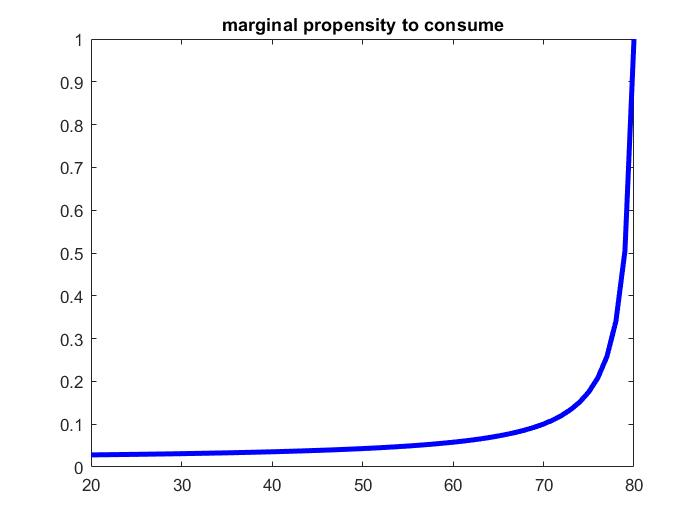
\includegraphics[width=8cm]{Pic1}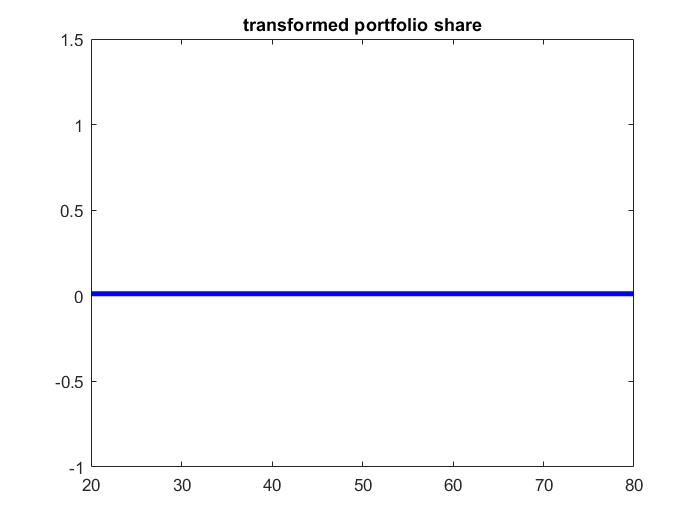
\includegraphics[width=8cm]{Pic2}\\
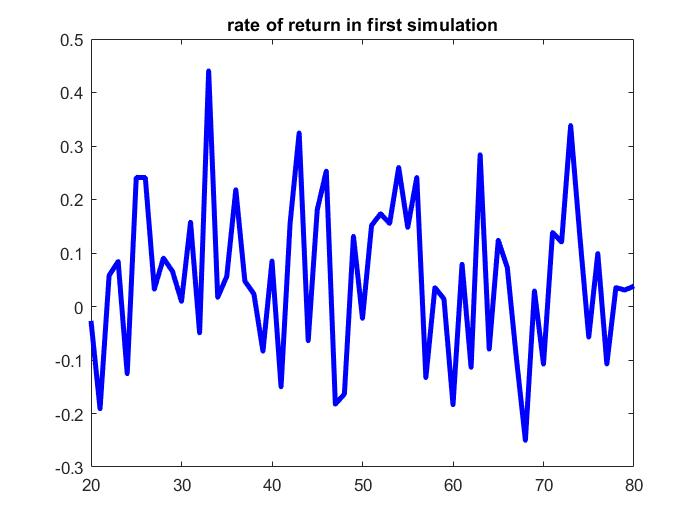
\includegraphics[width=8cm]{Pic3}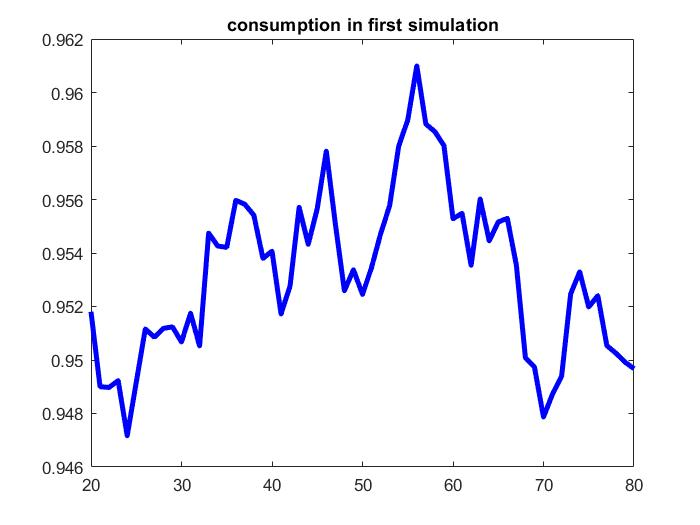
\includegraphics[width=8cm]{Pic4}\\
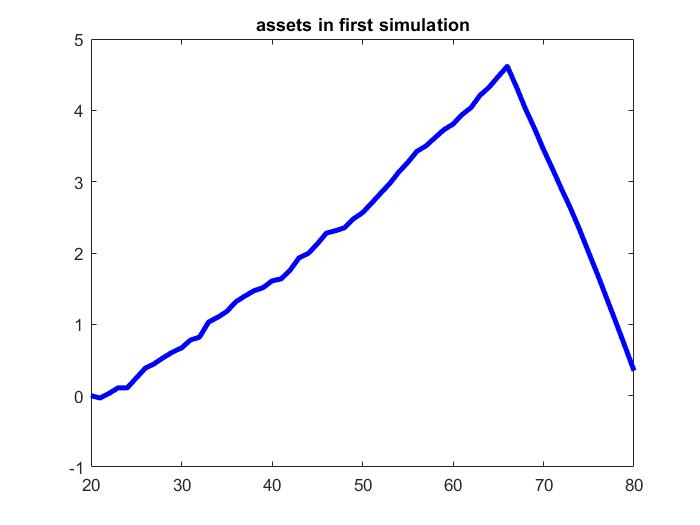
\includegraphics[width=8cm]{Pic5}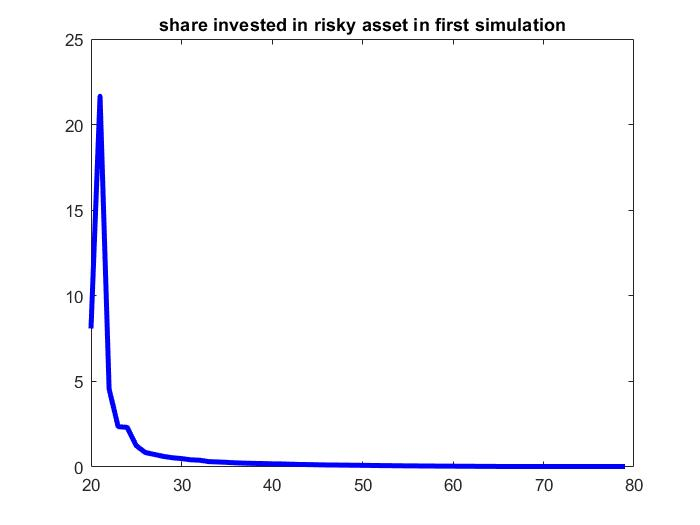
\includegraphics[width=8cm]{Pic6}\\
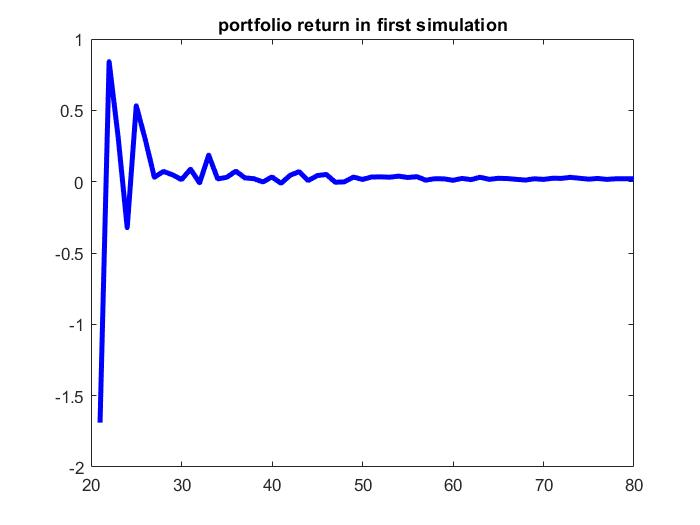
\includegraphics[width=8cm]{Pic7}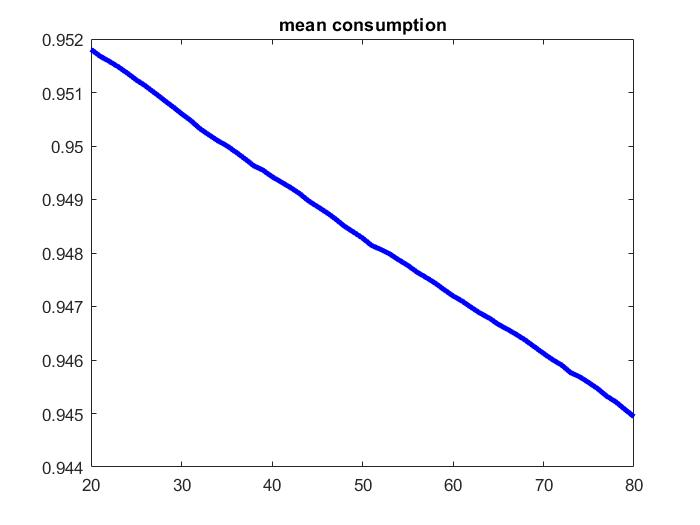
\includegraphics[width=8cm]{Pic8}\\
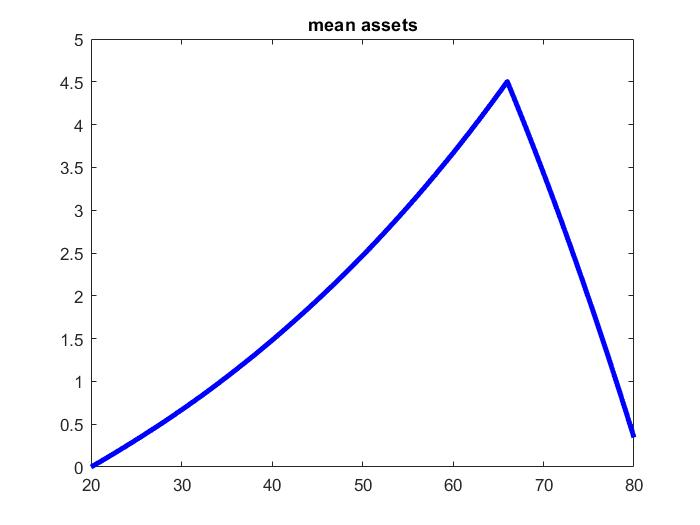
\includegraphics[width=8cm]{Pic9}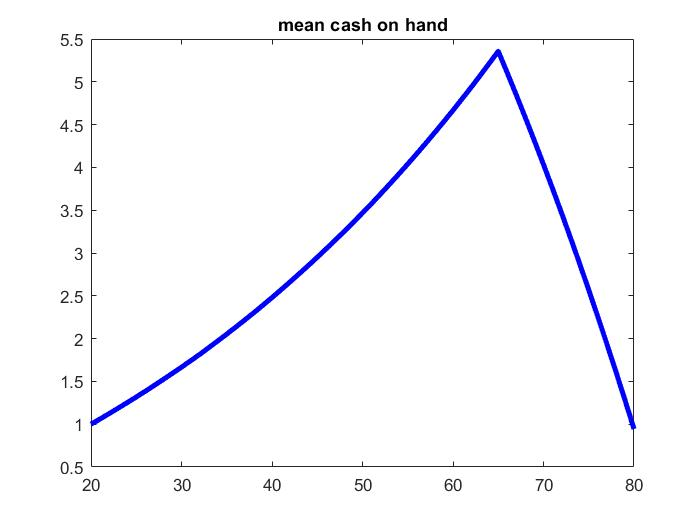
\includegraphics[width=8cm]{Pic10}\\
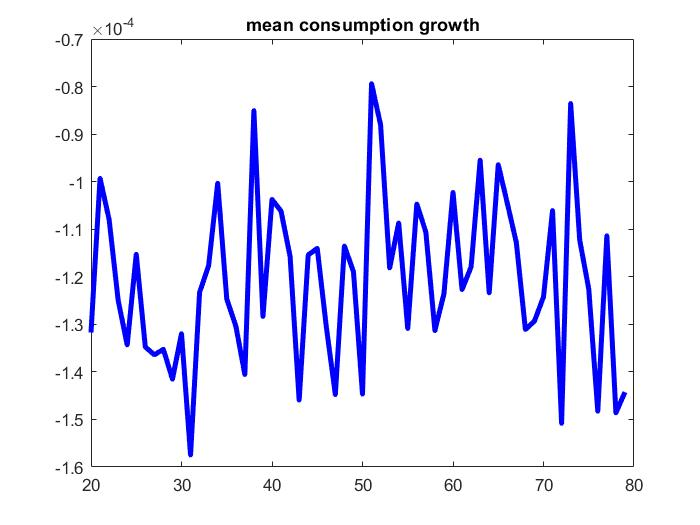
\includegraphics[width=8cm]{Pic11}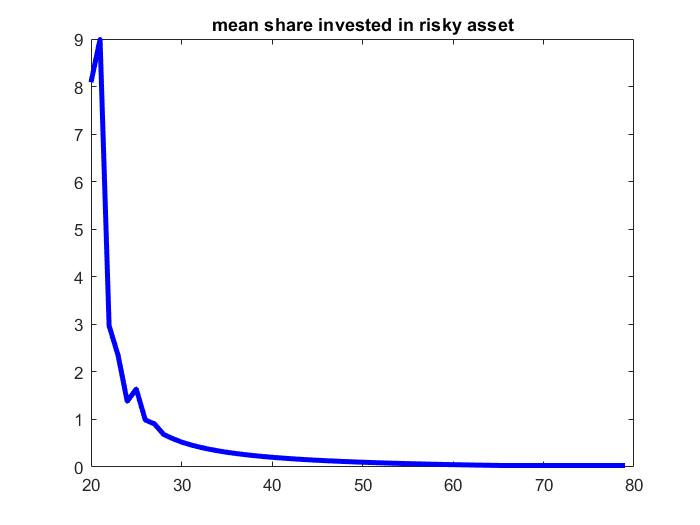
\includegraphics[width=8cm]{Pic12}\\
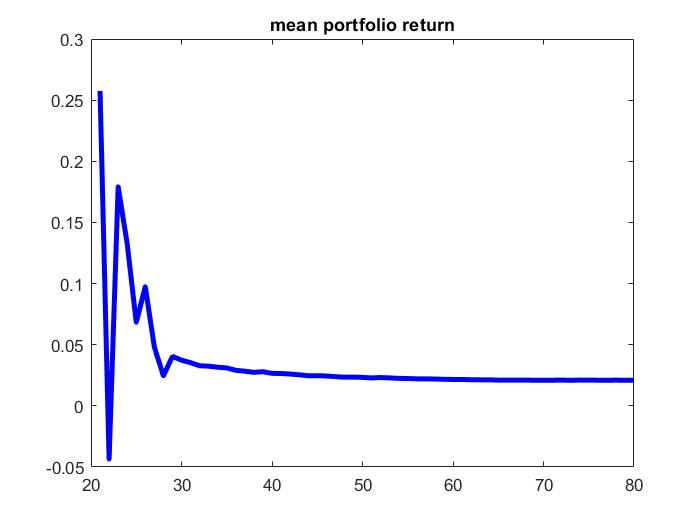
\includegraphics[width=8cm]{Pic13}
\end{center}
\textit{Pseudo code}\\

\begin{lstlisting}[frame=single]

% Main function for the life-cycle portfolio choice model:
begin function: life-cycle portfolio choice model

close all
 
% Set parameter values: 
discount rate = 0.02;
RRA = 150.0;
risk-free return = 0.02;          
mean risky return = 0.05;          
standard deviation of stock returns = 0.15;         
number of stochastic simulations = 10000;          
starting value cash at hands = 1.0;
net labour income during working period = 1.0;        
net replacement rate at retirement = 0.6;         
maximum age = 61;         
retirement age  = 46;          
 
% Transformation:
discount factor = 1 / (1+discount rate);
income = column vector of length maximum age filled with zeros;
change income(for year = 1 to year = retirement age) 
= net labour income during working period;
change income (for year = retirement age to year = maximum age) 
= net replacement rate at retirement * net labour income during working period;

% Policy functions:
function policy function output[marginal propensity to consume, estimated portfolio share] 
= input[maximum age, discount factor, RRA, risk-free return, mean risky return, 
standard deviation of stock returns];

% Human capital:
human capital = column vector of length maximum age filled with zeros;
for year = (maximum age - 1) until year = 1 {
change human capital(year) 
= [human capital (year + 1) + income (year + 1)] / (1 + risk-free return)
change year = year - 1;
}

% Plot policy functions:
% Remark: year = 1 is the first year an individual works
% Remark: year = maximum age is the last year an individual works
age vector = column vector of values 20 to (maximum age + 19);

plot(age vector on x-axis, marginal propensity to consume on y-axis);
plot(age vector on x-axis, estimated portfolio share on y-axis);

% Simulation:
initial state of random number generator = 0;

% Make space for simulated draws:
mean return = column vector of length maximum age filled with zeros;
mean estimated portfolio return = column vector of length maximum age filled with zeros;
mean portfolio return = column vector of length maximum age filled with zeros;
mean consumption = column vector of length maximum age filled with zeros;
mean portfolio share = column vector of length maximum age filled with zeros;
mean assets = column vector of length maximum age filled with zeros;
mean total wealth = column vector of length maximum age filled with zeros;
mean cash on hand = column vector of length maximum age filled with zeros;
mean total savings = column vector of length maximum age filled with zeros;
mean financial savings = column vector of length maximum age filled with zeros;
Rlong = empty array;


for simulation count = 1 until simulation count = number of stochastic simulations, {
log gross return = column vector of length maximum age filled with random numbers;
change log gross return 
= log gross return * standard deviation of stock returns + log(1.0+ mean risky return);
gross return = exp(log gross return + 0.5 * (standard deviation of stock returns) ^ 2);
simple return = gross return - 1.0;
Rlong =  Vector[Rlong;R];

Function fwdsolve output[consumption, consumption growth, cash on hands, assets, 
total wealth, total savings, financial savings, share invested in risky asset, 
estimated portfolio return, portfolio return]
= input[starting value of cash at hand, human capital, income, maximum age, 
marginal propensity to consume, portfolio share, risk-free return, simple return];

plot(age vector on x-axis, simple return on y-axis) if simulation count = 1;
plot(age vector on x-axis, consumption  on y-axis) if simulation count = 1;
plot(age vector on x-axis, assets  on y-axis) if simulation count = 1;
plot(age vector on x-axis, share invested in risky asset  on y-axis) if simulation count = 1;
% Remark: Return only from period 2 onwards:
plot(age vector(2:maximum age) on x-axis, portfolio return on y-axis) if simulation count = 1; 
    
% Calculate means (over simulations):
mean return = mean return + 1.0 / number of stochastic simulations * return;
mean portfolio return = mean portfolio return + 1.0 / number of stochastic simulations * portfolio return;
mean consumption = mean consumption + 1.0 / number of stochastic simulations * consumption;
mean assets = mean assets + 1.0 / number of stochastic simulations * assets;
mean total wealth = mean total wealth + 1.0 / number of stochastic simulations * total wealth;
mean cash on hand = mean cash on hand + 1.0 / number of stochastic simulations * cash on hand;
mean share invested in risky assets = mean share invested in risky assets + 1.0 / number of stochastic simulations * share invested in risky assets;
mean total savings = mean total savings + 1.0 / number of stochastic simulations * total savings;
mean financial savings = mean financial savings + 1.0 / number of stochastic simulations * financial savings;
}

plot(age vector on x-axis, mean consumption  on y-axis);
plot(age vector on x-axis, mean assets  on y-axis);
plot(age vector on x-axis, mean cash on hand  on y-axis);
plot(age vector on x-axis, mean assets  on y-axis);
% Remark: only (maximum age - 1) consumption growth values
pl=plot(agevec(1:nj-1),mcons(2:nj)./mcons(1:nj-1)-1.0,'b-');
plot(age vector on x-axis(1:(maximum age -1)), mean consumption(2:maximum age) divided elementwise by mean consumption (1:(maximum age - 1)) - 1.0 on y-axis);
plot(age vector on x-axis, mean share invested in risky asset on y-axis);
plot(age vector on x-axis, mean portfolio return on y-axis);

display ('THE END');
end function: life-cycle portfolio choice model

% Supplemental function for life-cycle portfolio choice model
begin function: policy function output[marginal propensity to consume; portfolio share] = input[maximum age, discount factor, discount rate, risk-free return, mean risky return, standard deviation of stock returns]

log mean risky return = log(1.0 + mean risky return);
marginal propensity to consume = column vector of length maximum age filled with ones;
estimated portfolio share = (log mean risky return-log(1.0+ risk-free return)+ standard deviation of stock returns ^2/2)/( RRA * standard deviation of stock returns ^2);
mup = estimated portfolio share * log mean risky return + (1-estimated portfolio share) * log(1+risk-free return) + 0.5 * estimated portfolio share * ( 1.0 - portfolio share) * variance of stock returns;
sigp = estimated portfolio share ^2 * standard deviation of stock returns ^2;

for year = (maximum age - 1) until year = 1{
% Calculate the marginal propensity to consume:
b = marginal propensity to consume(year+1) ^(-1) * (discount factor * exp ((1.0-RRA) * (mup + (1.0 - RRA) * sigp ^2/2))) ^(1/RRA);
marginal propensity to consume(year) = 1.0 / ( 1.0 + b);
change year = year - 1
}

end function: policy function

 % Supplemental function for life-cycle portfolio choice model
begin function: fwdsolve output[consumption, consumption growth, cash on hands, assets, total wealth, total savings, financial savings, share invested in risky asset, estimated portfolio return, portfolio return]=input[starting value cash at hand, human capital, income, maximum age, marginal propensity to consume, portfolio share, risk-free return, simple return];
% Make space for variable values: 
total savings = column vector of length maximum age filled with zeros;
financial savings = column vector of length maximum age filled with zeros;
cash on hands = column vector of length maximum age filled with zeros;
consumption = column vector of length maximum age filled with zeros;
assets = column vector of length maximum age filled with zeros;
total wealth = column vector of length maximum age filled with zeros;
portfolio share = column vector of length maximum age filled with zeros;
portfolio return = column vector of length maximum age filled with zeros;
estimated portfolio return = column vector of length maximum age filled with zeros;

cash on hands(year=1) = starting value of cash on hands;
total wealth (year=1) = starting value of cash on hands + human capital(year=1);

for year = 1 until year = maximum age, {
consumption(year) = marginal propensity to consume(year) * total wealth(year);
cash on hands(year)= total wealth(year)-human capital(year);
if year == 1, {
estimated portfolio return (year) = risk-free return + estimated portfolio share * (simple return(year)-risk-free return);
}

assets (year) = cash on hands (year) - income (year);

total savings(year) = total wealth (year) - consumption(year);
financial savings(year) = cash on hands (year) - consumption(year);

if year < maximum age, {
portfolio share (year) = estimated portfolio share * total savings(year)/financial savings(year);
estimated portfolio return (year + 1) = risk-free return + estimated portfolio share * ( simple return(year+1)-risk-free return);
portfolio return(year + 1) = risk-free return + portfolio share(year + 1) * (simple return(year + 1) - risk-free return);
total wealth (year + 1) = total savings (year) * ( 1+ estimated portfolio return (year + 1));
}
}

consumption growth = consumption(2:end) divided elementwise consumption (1:(end-1));

end function: fwdsolve


\end{lstlisting}


\textbf{Question 2}\\

\end{document}





